\documentclass[a4paper,11pt,fleqn]{article}%fleqn pour aligner les equations à gauche
\usepackage{../../Styles/Cours}


\newcommand{\chnum}{Chapitre 4}
\newcommand{\chtitle}{La Terre est sphérique !}
\newcommand{\dtype}{Act 1}


\begin{document}
\maketitle

Les interrogations sur la forme de la Terre remontent à la nuit des temps. Les premières hypothèses la supposent plate mais très vite, la sphéricité s'est imposée.

\begin{figure}[h!]
    \caption{Aristote et la Terre ronde}
    \begin{minipage}{.7\linewidth}
        La sphéricité de la terre est admise dès l'Antiquité par Aristote (384-322 av. J.-C.), pholosophe grac, disciple de Platon (428-348 av.J.-C.). Contrairement à une idée reçue, ce n'est pas Galilée (1564-1642) qui, le premier, a fait ce constat.\\
        En effet, Aristote avance des arguments physiques et empiriques. il s'appuie sur la forme circulaire de l'ombre portée de la Terre sur la Lune lors des éclipses. Il fait aiussi état des changements observés  dans l'aspect du ciel lorsqu'on va du Nord vers le Sud : des étoiles apparaissent, d'autres disparaissent.\\
        De plus, Aristote pense que la terre résulte de l'agglomération de ces composants sous l'effet d'une tendance naturelle des sobjets à se diriger vers un point central. de sorte que pour des raisons de symétrie naturelle des objets, elle ne peut posséder d'autres formes que sphérique.\\
        Dans son \emph{Traité du ciel} (livre II, chapitre 14), Aristore mentionne une estimation du périmètre de la Terre et insiste sur la petitesse de cette longueur par repport aux distances des corps cosmiques. Quelques années plus tard, Eratostène (276-194 av. J.-C.) détermine avec plus de précision la longueur de méridien terrestre.
    \end{minipage}
    \begin{minipage}{.28\linewidth}
        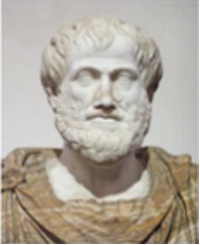
\includegraphics[width=\linewidth]{Ressources/1ES_C4_AE1_Fig1.png}
    \end{minipage}
\end{figure}

\begin{figure}[h!]
    \caption{L'éclipse de Lune du 27 juillet 2018}
    \begin{minipage} {.5\linewidth}
        En traversant l'atmosphère terrestre, les rayons du Soleil sont filtrés par l'atmosphère de la Terre, ce qui donne une couleur rouge à la Lune qu'on appelle \textit{Lune de sang} pour l'occasion. Ce phénomène a été observable depuis la France, particulièrement à l'Est du pays er sur l'île de La Réunion.
    \end{minipage}
    \begin{minipage}{.48\linewidth}
        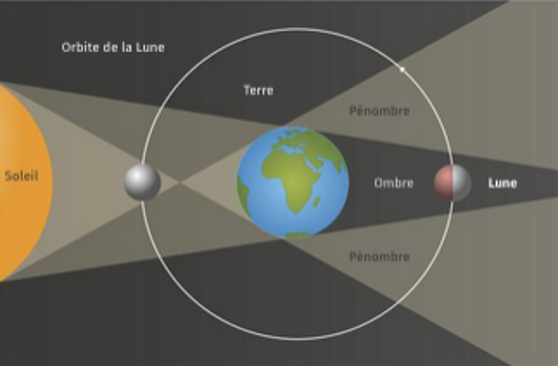
\includegraphics[width=\linewidth]{Ressources/1ES_C4_AE1_Fig2.png}
    \end{minipage}

    \begin{minipage}{\linewidth}
        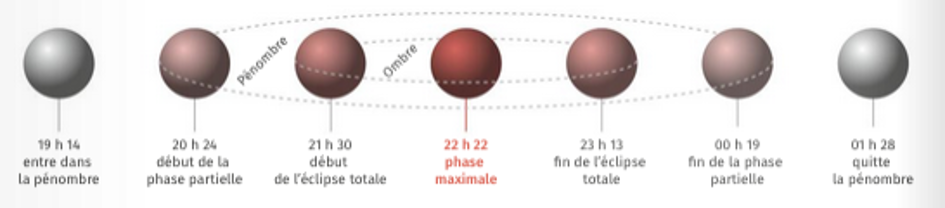
\includegraphics[width=\linewidth]{Ressources/1ES_C4_AE1_Fig3.png}
    \end{minipage}
\end{figure}

\newpage
\begin{figure}[h!]
    \caption{Apparence de la Lune à différents instants d'une éclipse}
    \begin{minipage}{\linewidth}
        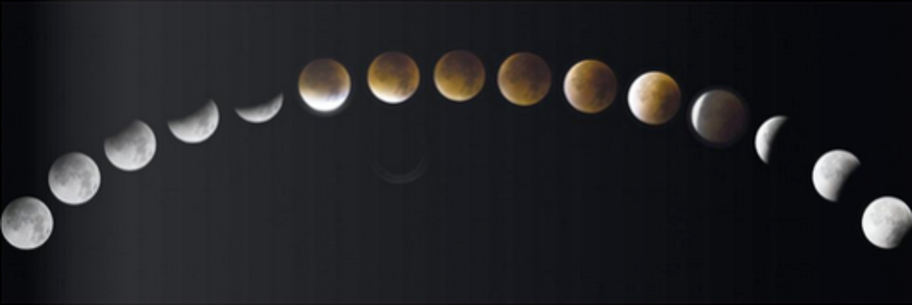
\includegraphics[width=\linewidth]{Ressources/1ES_C4_AE1_Fig4.png}
    \end{minipage}
\end{figure}

\begin{figure}[h!]
    \caption{La Terre change sans cesse de forme}
    \begin{minipage} {.5\linewidth}
        Répartition inégale des masse, épisode glaciaire ou réchauffement climatique modifient localement et au cours du temps la physionomie de notre planète.\\
        Avec son rayon de \SI{6371}{km}, la Terre est globalement ronde. Car il faut compter sur la répartition inégale des massses, aussi bien en surface que dans les profondeurs de la croûte et du manteau. Les matériaux qui la composent sont plus ou moins denses, certaines parties du manteau sont plus épaisses que d'autres ... autant de causes qui modifient localement le champ de gravité. Les mesures géodésiques réalisées ces dernières années montrent des bosses et des creux. la forme irrégulières de l'image est due aux effets de la gravité (les déformations ont été exagérées d'un facteur 100 000).
    \end{minipage}
    \begin{minipage}{.48\linewidth}
        \centering 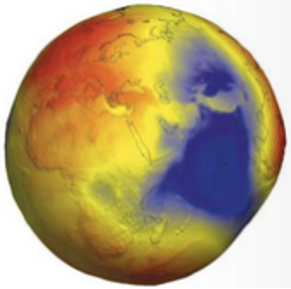
\includegraphics[width=.7\linewidth]{Ressources/1ES_C4_AE1_Fig5.png}
    \end{minipage}
\end{figure}

\textbf{Questions :}
\begin{enumerate}
    \item En quoi les arguments avancés par Aristote sont qualifiés d' "empiriques" ? (doc. 1)
    \item Quelles observations confortent Aristote dans l'idée que la terre est sphérique ? (doc. 1)
    \item Sur le schéma de l'éclipse lunaire, représentant les positions du Soleil, de la Terre et de la Lune, ajouter les sept formes de la Lune correspondant au déroulement de l'éclipse en les légendant avec des numéros. (doc. 3)
    \item Même s'il est admis que la terre est bien sphérique, à quoi sont dues les irrégularités dans sa sphéricité ? (doc. 4)
\end{enumerate}

\end{document}